\chapter{Дослідження стійкості різницевих алгоритмів для рівнянь з багатьма незалежними змінними}

\shortLectureDescription{Загальна схема дослідження. Відмінності в умовах стійкості різницевих схем для рівнянь дифузії-конвекції та повних рівнянь переносу}

\section{Метод фон Неймана для багатомірних задач}

Метод дискретних збурень (Томан і Шевчик [1966]) і метод Хьорта (Хьорт [1968]) можуть бути поширені на випадок дослідження стійкості в багатомірних задачах. Ми ж як приклад приведемо тут більш просте узагальнення методу Неймана на такий випадок. Використовуючи схему з різницями вперед за часом і із центральними різницями по просторовій змінній для лінеаризованого рівняння переносу вихору з постійними коефіцієнтами в плоскому випадку (коли $\alpha = 1 / \text{Re}$), одержуємо
\begin{multline}
    \label{eq:3.129}
    \frac{\zeta_{i, j}^{n + 1} - \zeta_{i, j}^n}{\Delta t} = -u \frac{\zeta_{i + 1, j}^n - \zeta_{i - 1, j}^n}{2 \Delta x} - v \frac{\zeta_{i, j + 1}^n - \zeta_{i, j - 1}^n}{2 \Delta y} + \\ + \alpha \left( \frac{\zeta_{i + 1, j}^n - 2 \zeta_{i, j}^n + \zeta_{i - 1, j}^n}{\Delta x^2} + \frac{\zeta_{i, j + 1}^n - 2 \zeta_{i, j}^n + \zeta_{i, j - 1}^n}{\Delta y^2} \right).
\end{multline}

Тепер запишемо кожну Фур'є-компоненту розв'язку у вигляді
\begin{equation}
    \label{eq:3.130}
    \zeta_{i, j}^n = V^n \exp\{ I (k_x i \Delta x + k_y j \Delta y) \}
\end{equation}
де $V^n$ знову є амплітудою на часовому шарі $n$ окремої Фур'є-компоненти, що має в напрямках $x$ і $y$ хвильові числа $k_x$ й $k_y$ (довжини хвиль $\Lambda_x = \frac{2 \pi}{k_x}$ і $\Lambda_y = \frac{2 \pi}{k_y}$), а $I = \sqrt{-1}$. \medskip

Уводячи фазові кути $\theta_x = k_x \Delta x$ й $\theta_y = k_y \Delta y$ для координат $x$ і $y$, запишемо вираз \eqref{eq:3.130} як
\begin{equation}
    \label{eq:3.131}
    \zeta_{i, j}^n = V^n \exp\{ I (i \theta_x + j \theta_y) \}
\end{equation}
аналогічно
\begin{equation}
    \label{eq:3.132}
    \zeta_{i + 1, j + 1}^{n + 1} = V^{n + 1} \exp\{ I ((i + 1) \theta_x + (j + 1) \theta_y)\}
\end{equation}
і т.д. 

\begin{definition}
    Відповідні двовимірні аналоги числа Куранта $C$ визначаються як $C_x = \frac{u \Delta t}{\Delta x}$ і $C_y = \frac{u \Delta t}{\Delta y}$, а відповідні аналоги величини $d$ як $d_x = \frac{\alpha \Delta t}{\Delta x^2}$ і $d_y = \frac{\alpha \Delta t}{\Delta y^2}$.
\end{definition}

Підставляючи ці величини у вираз \eqref{eq:3.130}, скорочуючи на спільний множник $\exp\{ I(i \theta_x + j \theta_y) \}$ і використовуючи формули Ейлера, знову одержуємо $V^{n + 1} = G V^n$, де
\begin{equation}
    \label{eq:3.133}
    G = 1 - 2 (d_x + d_y) + 2 d_x \cos \theta_x + 2 d_y \cos \theta_y - I (C_x \sin \theta_x + C_y \sin \theta_y).
\end{equation}

\begin{proposition}
    Очевидні необхідні умови виконання нерівності $|G| \le 1$ будуть
    \begin{equation}
        \label{eq:3.134}
        d_x + d_y \le \half,
    \end{equation}
    та
    \begin{equation}
        \label{eq:3.135}
        C_x + C_y \le 1.
    \end{equation}
\end{proposition}

\begin{example}
    В частинному випадку $d_x = d_y = d$ нерівність \eqref{eq:3.134} приймає вигляд
    \begin{equation}
        \label{eq:3.136}
        d \le \frac{1}{4}.
    \end{equation}
    
    Ця умова \emph{вдвічі сильніше} обмеження, отриманого для одномірного рівняння з одним тільки дифузійним членом. 
\end{example}

\begin{example}
    В частинному випадку $C_x = C_y = C$ нерівність \eqref{eq:3.135} приймає вигляд
    \begin{equation}
        \label{eq:3.137}
        C \le \half
    \end{equation}
    і знову виявляється \emph{вдвічі сильніше} відповідного необхідної умови в одномірному випадку.
\end{example}

\begin{remark}
    Фромм [1964] показав, що для частинного випадку $\Delta x = \Delta y = \Delta$ й $\theta_x = \theta_y = \theta$ обмеження на сіткове число Рейнольдса $\text{Re} = \frac{(|u| + |v|) \Delta}{\alpha}$ дається нерівністю
    \begin{equation}
        \label{eq:3.138}
        \text{Re}_{\text{с}} \le 4
    \end{equation}
    яке є \emph{менш жорстким}, ніж в одномірному випадку.
\end{remark}

\begin{exercise}
    Застосувати метод Неймана для дослідження стійкості схеми з різницями проти потоку для рівняння переносу у випадку нульової в'язкості
 	\begin{equation}
 	    \label{eq:3.139}
 	    \frac{\zeta_{i, j}^{n + 1} - \zeta_{i, j}^n}{\Delta t} = -u \frac{\zeta_{i, j}^n - \zeta_{i - 1, j}^n}{\Delta x} -v \frac{\zeta_{i, j}^n - \zeta_{i, j - 1}^n}{\Delta y}, \quad u > 0, \quad v > 0.
 	\end{equation}
    Показати, що умова стійкості має вигляд
 	\begin{equation}
 	    \label{eq:3.140}
 	    C_x + C_y \le 1.
 	\end{equation}
\end{exercise}

\begin{exercise}
    Застосувати метод Неймана до схеми з різницями вперед за часом і центральними різницями по просторових змінних для тривимірного рівняння дифузії
 	\begin{equation}
 	    \label{eq:3.141}
 	    \frac{\partial \zeta}{\partial t} = \alpha \left( \frac{\partial^2 \zeta}{\partial x^2} + \frac{\partial^2 \zeta}{\partial y^2} + \frac{\partial^2 \zeta}{\partial z^2} \right)
 	\end{equation}
    і показати, що умова
 	\begin{equation}
 	    \label{eq:3.142}
 	    d_x + d_y + d_z \le \half
 	\end{equation}
    є необхідною і достатньою для стійкості. В частинному випадку, коли $d_x = d_y = d_z = d$, умова \eqref{eq:3.142} має вигляд
 	\begin{equation}
 	    \label{eq:3.143}
 	    d \le \frac{1}{6}
 	\end{equation}
    і виявляється втричі жорсткіше, ніж в одномірному випадку.
\end{exercise}

\section{Однокрокові явні схеми. Схема ``чехарда із середньою точкою''}

Розглянута для лінійного модельного рівняння груба схема FTCS, що використовує різниці вперед за часом і центральні різниці по просторовим змінним, є однокроковою явною двошаровою за часом схемою. 

\begin{remark}
    \nothing
    \begin{itemize}
        \item Вона називається однокроковою, тому що для перехід до нового шару за часом потрібно тільки один обчислювальний крок. 
        \item Ця схема називається явною, тому що всі значення в правій частині 3.44.в, необхідні для обчислення $\zeta_i^{n + 1}$ на новому шарі за часом, відомі, тобто значення $\zeta_{i \pm 1}^{n + 1}$ не входять у праву частину рівняння.
        \item Вона є двошаровою за часом, тому що для обчислень тут залучаються тільки два шари за часом; нові значення на шарі $n + 1$ обчислюються тільки за значеннями на шарі $n$.
    \end{itemize}
\end{remark}

Схема із центральними різницями по просторових змінних і за часом, яка, як уже було відзначено, безумовно нестійка при будь-яких $\alpha > 0$ і $\Delta t > 0$. Але при застосуванні тільки до конвективних членів (тобто при $\alpha = 0$) ця схема, називана схемою із середньою точкою (Ліллі [1965]) або схемою ``чехарда із середньою точкою'' або --- найчастіше --- просто ``чехарда'' (Курант, Фрідріхс, Леві [1928]), має потрібні властивості стійкості. 

\begin{example}
    Таким чином, рівняння
    \begin{equation}
        \label{eq:3.144}
        \frac{\partial \zeta}{\partial t} = -\frac{\partial(u \zeta)}{\partial x}
    \end{equation}
    за цією схемою представляється у вигляді
    \begin{equation}
        \label{eq:3.145}
        \frac{\zeta_i^{n + 1} - \zeta_i^{n - 1}}{2 \Delta t} = -\frac{(u \zeta)_{i + 1}^n - (u \zeta)_{i - 1}^n}{2 \Delta x}.
    \end{equation}
\end{example}

\begin{proposition}
    Дана схема має другий порядок точності по просторі й за часом.
\end{proposition}

Це однокрокова явна тришарова за часом схема. Виходить, для обчислення нових значень на шарі $n + 1$ в цій схемі необхідні значення на шарах $n$ і $n - 1$. 

\begin{remark}
    Помітимо, що нові $\zeta$ на парному часовому шарі обчислюються як значення $\zeta$ на попередньому парному часовому шарі плюс деяке збільшення, а попередній непарний часовий шар при цьому ``перестрибається'' (звідси й назва схеми --- ``чехарда'').
\end{remark}

Метод фон Неймана дослідження стійкості для цієї й інших багатошарових схем застосовується в такий спосіб. Використовуючи ті ж визначення й припущення, що й у попередніх прикладах, рівняння \eqref{eq:3.145} можна записати в наступному виді:
\begin{equation}
    \label{eq:3.146}
    \zeta_i^{n + 1} = \zeta_i^{n - 1} - C (\zeta_{i + 1}^n - \zeta_{i - 1}^n),
\end{equation}
де $C = \frac{u \Delta y}{\Delta x}$ --- число Куранта. Підставляючи сюди фур'є-компоненти, 
одержуємо зв'язок для амплітуд 
\begin{equation}
    \label{eq:3.147}
    V^{n + 1} = a V^n + V^{n - 1},
\end{equation}
де
\begin{equation}
    \label{eq:3.148}
    a = -2/C \sin \theta.
\end{equation}

Щоб одержати матричне рівняння, додамо до \eqref{eq:3.147} тотожність
\begin{equation}
    \label{eq:3.149}
    V^n = 1 \cdot V^n + 0 \cdot V^{n + 1}.
\end{equation}

Розглядаючи це рівняння разом з рівнянням \eqref{eq:3.147} одержуємо
\begin{equation}
    \label{eq:3.150}
    \begin{pmatrix}
        V^{n + 1} \\ V^n
    \end{pmatrix}
    = G
    \begin{pmatrix}
        V^n \\ V^{n - 1},
    \end{pmatrix}
\end{equation}
де множник переходу $G$ тепер являє собою матрицю
\begin{equation}
    \label{eq:3.151}
    G = \begin{pmatrix}
        a & 1 \\ 1 & 0
    \end{pmatrix}
\end{equation}

Для вивченої раніше одношарової схеми множник переходу $G$ був просто числом, а умова стійкості мала вигляд $|G| \le 1$. 

\begin{proposition}
    У випадку ж, коли $G$ являє собою матрицю, умову стійкості (згідно фон Нейману) має такий вигляд:
    \begin{equation}
        \label{eq:3.152}
        |\lambda| \le 1,
    \end{equation}
    де $\lambda$ --- усі можливі власні значення матриці $G$. 
\end{proposition}

\begin{remark}
    Власне значення до матриці визначається як корінь характеристичного рівняння, яке утворюється прирівнюванням до нуля визначника матриці, у якого з кожного діагонального елемента віднімається $\lambda$). Таким чином, характеристичне рівняння для визначення матриці $G$ записується так:
 	\begin{equation}
 	    \label{eq:3.153}
 	    \begin{vmatrix}
 	        a - \lambda & 1 \\ 1 & 0 - \lambda
 	    \end{vmatrix} = 0.
 	\end{equation}
\end{remark}

Коли $G$ являє собою просте число, як у попередніх прикладах, воно розглядається як одномірна матриця. Тоді рівняння для визначення власного значення приймає вигляд $G - \lambda = 0$ або $\lambda = G$, тому умова \eqref{eq:3.152} зведеться до попередньої умови $|G| \le 1$.) Розкриваючи визначник і розв'язуючи отримане квадратне рівняння відносно $\lambda$, знаходимо два розв'язки:
\begin{equation}
    \label{eq:3.154}
    \lambda_\pm = \half ( a \pm \sqrt{a^2 + 4} ).
\end{equation}

Враховуючи, що $a = -2 I C \sin \theta$ й $a^2 = -4 C^2 \sin^2 \theta$, маємо
\begin{equation}
    \label{eq:3.155}
    \lambda_\pm = -I C \sin \theta \pm \sqrt{1 - C^2 \sin^2 \theta}.
\end{equation}

У тих випадках, коли $C^2 \sin^2 \theta \le 1$, підкореневий вираз буде від’ємним, і тоді
\begin{equation}
    \label{eq:3.156}
    \lambda_\pm = I \left( -C \sin \theta \pm \sqrt{C^2 \sin^2 \theta - 1} \right).
\end{equation}

При цьому абсолютна величина $|\lambda| > 1$, що означає нестійкість. У тому ж випадку, коли $C^2 \sin^2 \theta \le 1$, для чого, загалом кажучи, потрібне виконання 
умови
\begin{equation}
    \label{eq:3.157}
    C \le 1
\end{equation}
одержуємо
\begin{align}
    \label{eq:3.158}
    |\lambda_\pm|^2 &= C^2 \sin^2 \theta + (1 - C^2 \sin^2 \theta), \\
    \label{eq:3.159}
    |\lambda_\pm| &= 1, \quad C \le 1.
\end{align}

Це задовольняє умові стійкості \eqref{eq:3.152} у граничному випадку рівності. Аналогічний результат виходить також при двох просторових змінних, але тут для стійкості потрібне виконання нерівності $C_x + C_y \le 1$. \medskip

Можна подумати, що, значення $|\lambda_\pm| = 1$ з \eqref{eq:3.159}, що відповідає границі стійкості, є прийнятним лише в крайньому випадку, але в дійсності це значення навіть досить бажане, якщо розв'язок вихідного диференціального рівняння не є загасаючим. Насправді, рівняння конвекції \eqref{eq:3.144} при відсутності в'язкості й постійному $u$ виражає той факт, що довільний початковий розподіл функції $\zeta(x, 0)$ просто зсувається зі швидкістю конвекції $u$; виходить, для будь-якого зсуву $\tau$ за часом розв'язок цього рівняння має вигляд
\begin{equation}
    \label{eq:3.160}
    \zeta(x, t + \tau) = \zeta(x - u \tau, t).
\end{equation}

Таким чином, метод фон Неймана показує, що схема ``чехарда'' правильно моделює одну із властивостей, властивих розв'язку вихідного диференціального рівняння при $u = \const$, а саме відсутність загасання. Будь-яка різницева схема для розв'язку рівняння для нев'язкої рідини, така, що $|G| < 1$, має помилку, обумовлену штучним або чисельним загасанням. У будь-якій збіжній різницевій схемі ця помилка повинна, звичайно, прямувати до нуля при $\Delta x \to 0$, $\Delta t \to 0$, але застосування методу фон Неймана показує, що схема ``чехарда'' при $u = \const$ й $C \le 1$ має нульову похибку, обумовлену загасанням, навіть при скінченних $\Delta x$ і $\Delta y$. \medskip

Дійсно, в частинному випадку $C = 1$ розглянута схема дає точні результати. Поклавши $\tau = \Delta t$, маємо $x - u \tau = x - C \Delta x$, тому при $C = 1$ розв'язок \eqref{eq:3.160} можна переписати так:
\begin{equation}
    \label{eq:3.161}
    \zeta_i^{n + 1} = \zeta_{i - 1}^n.
\end{equation}

Отже, точний розв'язок диференціального рівняння, якщо його розглядати у вузлових точках кінцево-різницевої сітки, виражає перенос величини $\zeta$ із точки $i - 1$ на шарі $n$ в точку  $i$ на шарі $n + 1$. Величина $\zeta$ за один крок за часом переноситься з конвективною швидкістю $u$ на відстань $u \Delta t$, а при $C = 1$ відстань $u \Delta t$ рівна $\Delta x$. Через два часові кроки точний розв'язок буде
\begin{equation}
    \label{eq:3.162}
    \zeta_i^{n + 1} = \zeta_{i - 2}^{n - 1}.
\end{equation}

У результаті застосування схеми ``чехарда'' \eqref{eq:3.146} при $C = 1$ одержуємо
\begin{equation}
    \label{eq:3.163}
    \zeta_i^{n + 1} = \zeta_i^{n - 1} - \zeta_{i + 1}^n + \zeta_{i - 1}^n.
\end{equation}

Задавши правильні початкові значення згідно з рівнянням \eqref{eq:3.161}, а саме $\zeta_{i + 1}^n = \zeta_i^{n - 1}$ й $\zeta_{i - 1}^n = \zeta_{i - 2}^{n - 1}$, одержуємо, що різницевий розв'язок \eqref{eq:3.163} збігається з точним розв'язком \eqref{eq:3.162}. Таким чином, при $u = \const$ й $C = 1$ схема ``чехарда'' дає точний розв'язок.

\begin{remark}
    Однак при практичних гідродинамічних розрахунках, коли швидкість змінюється в просторі, обмеження на крок $\Delta t$ буде визначатися (якщо не враховувати додаткові ускладнення, обумовлені нелінійністю) найбільшим значенням $u$ у вузлових точках сітки. Виходить, загалом кажучи, не можна одержати $C = 1$ у всіх точках. Але при $C < 1$ різницева схема ``чехарда'' вже не буде давати точного розв'язку.
\end{remark}

Насамперед всупереч результатам методу фон Неймана розглянутій схемі може бути притаманно певне чисельне загасання, хоча це звичайно не допускається. На мал.~\ref{fig:3.10} представлені тривимірні графіки величини $\zeta(x, t)$, розрахованої за схемою ``чехарда'' при синусоідально мінливій на вхідній границі потоку величині $\zeta(0, t) = \sin t$. При $C = 1$, як видно на мал.~\ref{fig:3.10}.а, отримується точний розв'язок із синусоїдальним законом на вхідній границі, який переноситься за рахунок конвекції без загасання. На мал.~\ref{fig:3.10}.б побудована діаграма, розрахована із удвічі меншим кроком за часом, тобто при $C = \half$. Видно, що в цьому випадку максимум амплітуди першого горба зменшується при русі вниз за потоком. Мал.~\ref{fig:3.10}.в знову відповідає $C = \half$, але період зміни $\zeta$ на вхідній границі й величина кроку за часом обрані таким чином, щоб їх відношення (і крок $\Delta x$) були такими ж, як і для мал.~\ref{fig:3.10}.а; у цьому випадку загасання дуже сильне.
 
\begin{figure}[H]
    \centering
    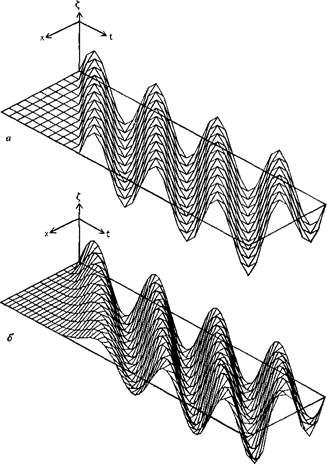
\includegraphics[width=.3\textwidth]{{img/08/3.10.ab}.png} \qquad
    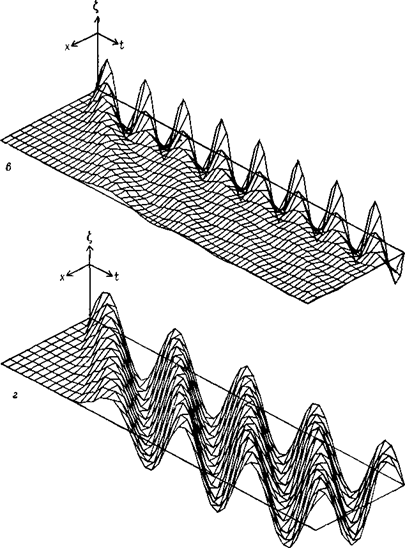
\includegraphics[width=.3\textwidth]{{img/08/3.10.cd}.png}
    \caption{[У. Сандберг]. Розв'язки рівняння $\frac{\partial \zeta}{\partial t} = -\frac{u \partial \zeta}{\partial x}$, отримані за допомогою схеми ``чехарда''. Тут $C$ --- число Куранта, $N$ --- сіткова частота. а: $C = 1$, $N = 8$; б: $C = \half$, $N = 16$; в: $C = \half$, $N = 8$; г: $C = \frac{3}{4}$, $N = 10.667$.}
    \label{fig:3.10}
\end{figure}

\begin{remark}
    Тут виникає питання щодо застосування терміна ``загасання''. Метод фон Неймана став настільки широко відомим, що ``загасання'' звичайне розуміється в значенні поведінки Фур'є-компонентів як випадок, коли $|\lambda| < 1$. Очевидно, якщо термін ``загасання'' означає по визначенню, що $|\lambda| < 1$ , то схема ``чехарда'' по визначенню не має загасання.
\end{remark}

Зменшення ж екстремальних величин амплітуди, яке видно на мал.~\ref{fig:3.10}.б і \ref{fig:3.10}.в, правильно пов'язувати з дисперсійною помилкою, яка проявляється в методі фон Неймана й буде коротко обговорюватися надалі. Така термінологія доцільна, і її можна навіть рекомендувати в тих випадках, коли мається на увазі, що схема насправді може викликати зменшення екстремальних величин амплітуд хвиль. Звичайно таку властивість називають ``загасанням''; що ж стосується мал.~\ref{fig:3.10}.в, то краще було б говорити, що хвиля не загасає, а зменшує свою амплітуду в міру її переносу за рахунок конвекції. \medskip

Ґрунтуючись на мал.~\ref{fig:3.10} можна зробити й інший висновок. При розв'язанні скін\-чен\-но-різ\-ни\-це\-вих рівнянь для задач, аналогічних представленої на мал.~\ref{fig:3.10} існує два характеристичні параметри. Перший параметр являє собою число Куранта, яке є єдиним параметром при розв'язку скінчено-різницевого рівняння у внутрішніх точках. Другим параметром є сіткова частота$N = \frac{2 \pi}{\Delta t}$, тобто число часових шарів за період зміни функції на вхідній границі потоку. \medskip

Порівняння мал.~\ref{fig:3.10}.б і \ref{fig:3.10}.в приводить до висновку, що для фіксованого $C < 1$ загасання (зменшення екстремальних амплітуд) послабляється зі збільшенням сіткової частоти в тому випадку, коли сіткова частота $N$ являє собою ціле число. Але коли $N$ не є цілим числом (випадок, зображений на мал.~\ref{fig:3.10}.г), то відбувається ``недозагасання'' амплітуди; як показано на мал.~\ref{fig:3.10}.г, амплітуди ``недозагасають'' на 15\% від амплітуди піка на вхідній границі, що обумовлене фазовими помилками. Даний ефект не можна повністю спасити на рахунок умови на вихідній границі потоку; уже до того, як почується який-небудь вплив цих умов, спостерігається недозагасання амплітуди на 8\%. \medskip

Схемі ``чехарда'' властиві також інші помилки й аномалії. Диференціальне рівняння \eqref{eq:3.144} є рівнянням першого порядку по просторових змінних і за часом; для всіх $x > 0$, $t > 0$ розв'язок повністю визначається завданням початкових умов $\zeta(x, 0)$ і граничних умов $\zeta(0, t)$. Але для початку обчислень за допомогою дискретного аналога \eqref{eq:3.145} потрібно два набори початкових умов, тому що для розрахунків значень на $(n+1)$-ому шарі необхідні значення на $n$-ому і $(n-1)$-ому шарах. \medskip

Таким чином, скінчено-різницеве рівняння фактично є рівнянням другого порядку за часом і вимагає початкових умов $\zeta_i^1$ і $\zeta_i^2$. Це аналогічно завданню початкових значень $\zeta(x, 0)$ і $\left. \frac{\partial \zeta}{\partial t}\right|_{t = 0}$ для диференціального рівняння, що робить задачу для диференціального рівняння перевизначеною. Для одержання $\zeta_i^2$ повинна бути використана інша ``розгінна'' скінчено-різницева схема, після чого можна застосовувати схему ``чехарда''. Якщо така ``розгінна'' схема дає точні результати, як це передбачалося після обговорення рівняння \eqref{eq:3.163}, то й наступний розв'язок за схемою ``чехарда'' при $C = 1$ буде точним. Якщо ж ``розгінна'' схема вносить помилку в значення $\zeta_i^2$, то ця помилка буде зберігатися при наступних розрахунках за схемою ``чехарда''. \medskip

Таким чином, правильніше казати, що схема ``чехарда'' при $C = 1$ зберігає, а не дає точний розв'язок, заданий на першому часовому шарі, для всіх часових шарів. \medskip

Іншим типом помилки схеми ``чехарда'' (і всіх інших схем) при $C = 1$ є фазова помилка. При розв'язанні диференціального рівняння весь початковий розподіл $\zeta(x, 0)$ поширюється зі швидкістю конвекції $u$. При скінчено-різницевих розрахунках різні Фур'є-компоненти мають різні швидкості конвекції, причому швидкість компонентів з найбільшою довжиною хвилі $\Lambda$ наближається до правильного значення $u$, а компоненти з меншими довжинами хвиль поширюються з меншими швидкостями. Це явище легко продемонструвати, розглядаючи (див. мал.~\ref{fig:3.11}) найменшу можливу довжину хвилі $\Lambda = 2 \Delta x$ на просторовій сітці нескінченної довжини. Для загальності збурення на $(n - 1)$-му і $n$-му часових шарах узяті з різними амплітудами, що відповідає використанню ``розгінної'' схеми, для якої не виконується умова $G = 1$.

\begin{figure}[H]
    \centering
    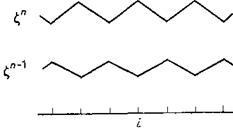
\includegraphics[width=.25\textwidth]{{img/08/3.11}.png}
    \caption{Фур'є-компонента з довжиною хвилі $\Lambda = 2 \Delta x$ на просторовій сітці нескінченної довжини.}
    \label{fig:3.11}
\end{figure}

З мал.~\ref{fig:3.11} ясно, що
\begin{equation}
    \label{eq:3.164}
    \left. \frac{\delta \zeta}{\delta t} \right|_i^n = \frac{\zeta_{i + 1}^n - \zeta_{i - 1}^n}{2 \Delta x} = 0
\end{equation}
для всіх $i$. Таким чином, $\zeta_i^{n + 1} = \zeta_i^{n - 1}$ і $\zeta_i^{n + 2} = \zeta_i^n$ і т.д. Виходить, тут має місце чергування двох штучно заданих початкових розподілів з довільною амплітудою. Фур'є-компонента з довжиною хвилі $\Lambda = 2 \Delta x$ є повністю стаціонарною, причому має місце повна помилка фазової швидкості. \medskip

Ця поведінка узгоджується з тим фактом, що схема ``чехарда'' при $C = 1$ зберігає точний розв'язок. Якщо почати розрахунки з точного розв'язку $\zeta_i^n = \zeta_{i - 1}^n$, то для компоненти з $\Lambda = 2 \Delta x$ наступний правильний розв'язок насправді буде $\zeta_i^{n + 1} = \zeta_{i - 2}^{n - 1} = \zeta_i^{n - 1}$. Ясно, що, хоча схема ``чехарда'' має другий порядок точності, у дійсності точність визначається точністю ``розгінної'' схеми, що використовується на початковій стадії розрахунків. \medskip

Схема ``чехарда'', розглянута для конвективних членів, застосовна також для течій з малими $\text{Re}$ (Хин і Макано [1966]) і для течій нев'язкої рідини за умови, що точний початковий розв'язок розраховується окремо й що стаціонарний стан не досягається. \medskip

У схемі ``чехарда'' (і у всіх схемах другого порядку точності із центральними різницями по просторових змінних) мають місце й додаткові помилки. Розглянемо скінчено-різницеву схему, у якої найбільше значення $i$ рівно $IL$. Застосування схеми ``чехарда'' \eqref{eq:3.145} для обчислення $\zeta_{IL}^{n + 1}$  вимагало б значення величини $\zeta_{IL + 1}^{n + 1}$ в точці, яка перебуває поза розрахунковою сіткою. Тому в точці $IL$ не можна провести розрахунки й для визначення потрібно задати чисельну граничну умову в $IL$. \medskip

Така вимога аналогічна необхідності задання двох наборів початкових умов і веде до перевизначеності задачі для диференціального рівняння. Помітимо також, що звичайно використовувана умова рівності нулю градієнта для задання умови на вхідній границі потоку, коли вважаються $\zeta_{IL}^{n + 1} = \zeta_{IL + 1}^{n + 1}$ приводить до руху стаціонарної (в інших відносинах) фур'є-компоненти з довжиною хвилі $\Lambda = 2 \Delta x$, але цей рух не має нічого спільного з тим, що відбувається при конвекції. З ростом часу ця фур'є-компонента із $\Lambda = 2 \Delta x$ загасає по сітці зправа (від вихідної границі потоку) наліво, тоді як справжня конвекція розвивається зліва направо. \medskip

Така неправильна вимога, що полягає в заданні додаткової умови на вихідній границі потоку, є наслідком помилки ще одного виду, а саме обумовленої порушенням властивості транспортивності. \medskip

\begin{exercise}
    За допомогою обчислень вручну й геометричних міркувань перевірити, що схема ``чехарда'' дає правильну поведінку розв'язку на лівій границі (вхідна границя потоку). Задавши початкову умову, що включає тільки компоненту з $\lambda = 2 \Delta x$, і зафіксувавши граничну умову на вхідній границі потоку для всіх моментів часу, почати розрахунки за схемою ``чехарда'' при $C = 1$ при точному розв'язку на другому тимчасовому шарі. Показати, що при $C = 1$ початковий профіль правильно поширюється по сітці.
\end{exercise}

Слід також помітити, що назва ``чехарда'' застосовується для багатьох схем, що відрізняються видом апроксимації просторових похідних, але всі вони є тришаровими й використовують центральні різниці за часом, як і тільки що розглянута схема.

\section{Завдання для самостійної роботи}

\shortHomeworkDescription{Побудувати апріорну оцінку кількості арифметичних операцій при використанні явних та неявних різницевих алгоритмів знаходження розв'язків дво- і трьохвимірних рівнянь переносу.}
